\documentclass{article}
\usepackage{amsmath, graphicx, amsfonts, caption, subfig, keyval, algorithm, algorithmic}
\captionsetup{justification=centering}
\newcommand{\R}{\mathbb{R}}
\newcommand{\C}{\mathcal{C}}
\newcommand{\X}{\mathcal{X}}
\DeclareMathOperator*{\argmin}{\arg\!\min}

\begin{document}
\title{Weighted $k$-Centers \& Lloyd's Algorithm}
\author{Jonathan Friedman \& Taylor Killian}
\maketitle

\begin{abstract}
When determining the optimal location of distribution centers (e.g. warehouses, regional retail, or neighborhood commercial property), consideration must be made to provide effective customer service. It is assumed that individuals prefer the distance from them to any distribution center be minimized. To select the optimal location of distribution centers that minimize the average person's distance from any center, Lloyd's algorithm was modified to solve a variant of weighted $k$-centers. This augmented clustering algorithm is used to simulate a variety of distribution paradigms (differentiated by the weighting function used) using the 2010 U.S. Census population data for Massachusetts which provides a dense decision surface to optimize over. Results reaffirm the intuition that dense areas of high population are optimal locations to place centers. The effects of various weighting functions and population filterings on center locations are discussed.

\end{abstract}

\section{Introduction} \label{introduction}
Serving the maximum number of people at minimum expense is a canonical problem in the retail and commercial industries. A company must balance placing their distribution centers near as many people as possible with the cost associated with opening and maintaining a large number of centers. A general formulation of this problem known as the metric $k$-center problem asks for a placement of $n$ distribution centers that minimizes the maximum distance from any point to a center \cite{kmeans}. In this paper, we examine the variant in which each point has a weight that affects its distance from the center point; for this report the weight is considered to be a function of the population at each point. We also seek to minimize the sum of the maximum distances rather than the maximum individual distance. Efficient algorithms to solve this problem exist in one dimension \cite{1D}. For the two-dimensional case, we adapt Lloyd's algorithm, an algorithm commonly used to find evenly spaced points and subsets within a given set of data, to work on the 2010 U.S. Census data from the state of Massachusetts by modifying the clustering step. 

If no attempt is made to avoid local extrema, then this problem is easy to solve for one center. In section \ref{onecenter}, we give a solution for one center using compass search. However, compass search is not viable for a large number of points because the number of required directions to search grows quickly. In section \ref{multicenters}, we give a solution method for an arbitrary number of centers using the variant on Lloyd's algorithm. In section \ref{experiments}, we use our algorithm to optimize placement of distribution centers in the population data of Massachusetts, subject to different constraints. We considered the use of various weighting functions centers, as well as the use of population filtering.

\section{Background \& Data} \label{background}
\subsection{Background}
Let $\C$ be the set of distribution centers, let $\X$ be the set of points which the centers serve, and let $d$ be a distance metric. In the general metric $k$-center problem, the goal is to minimize

$$\max_{p_i \in \X} \min_{c \in \C} d(c, p_i)$$

Now let $\xi_i$ be the population at point $p_i \in \X$, and $w: \X \rightarrow \R^{|\X|}$ be a weight function (we consider only weight functions where $\xi_i > \xi_j \implies w(\xi_i) \geq w(\xi_j)$, though more exotic functions could be useful in other contexts). In the version of the weighted $k$-center problem that we consider, the goal is to minimize our cost function, the ``weighted mean distance" function

$$\frac{\sum_i w(\xi_i) \min_{c \in \C} d(c, p_i)}{|\X|}$$

Note that while the minimum achieved in the standard metric $k$-center problem corresponds to distance, the minimum achieved in the weighted problem does not have a consistent physical interpretation across all weighting functions. When $w$ is the identity function, it corresponds to minimizing the distance from the average population center, rather than the average point, to its nearest distribution center. In general, it can be intuitively thought of as a weighted analogue to this mean distance, but its precise interpretation depends on the domain and context of the problem.

The choice of $w$ is also context and domain dependent, as shown below in Section \ref{experiments}. See section \ref{results} for further discussion.

Unless otherwise specified, $d$ is the standard Euclidean distance. Of course, this distance metric does not capture the true surface distance between points on the Earth. Since we test our algorithm on geographic data, we should, strictly speaking, use a different distance function such as the haversine formula. Euclidean distance provides a good approximation on sufficiently small regions, such as the state of Massachusetts, for which the curvature of the Earth is negligible when calculating the distance between two points.

We also consider the use of a population filter to ignore points below a given population. We call $p: \R\rightarrow\R$ a population filter if, for some $n \in \mathbb{N}$,

$$p(\xi)=\begin{cases}\xi, & \xi \geq n\\ 0, & \text{otherwise} \end{cases}$$

When applied to a space $\X$, such a $p$ transforms the space into one where all points with $\xi<n$ are ignored. Decreasing the number of points in the space could speed computation on large datasets for which considering every point is prohibitively expensive. It is not necessary in our case, but we investigate its effect on center locations.

\subsection{Related Work}
There are no efficient algorithms known for the weighted $k$-centers problem in two dimensions \cite{kmeans}. Chen et. al. give a simple $\mathcal{O}(n \log n)$ algorithm for the one-dimensional case \cite{1D}, but this approach is not known to be generalizable to higher dimensions. Various algorithms for solving weighted clustering problems are discussed in \cite{weightedclustering}, and Lloyd's algorithm has been generalized to solve crystal lattice problems \cite{crystal} but we are not aware of applications of Lloyd's algorithm to our specific problem.

\subsection{Census Data}
Throughout the paper, we test our algorithms using census block population data for Massachusetts from the 2010 U.S. Census. A census block is the smallest geographic unit for which population data is collected for every resident. Population data on a block level is available at \cite{census}, and can be parsed using geographic information software such as the Python Shapefile Library \cite{pyshp}. To generate a representative point for each block, we enclose the block in a bounding rectangle, then take the center of that rectangle to be the location of the block.

Although the 2010 Census divided Massachusetts into 157,508 total census blocks, 61,174 of those blocks have a population of zero (since every point in the United States is within a census block, many of which are often delimited by geophysical features, several blocks are located in lakes, national parks, shopping malls, and so forth) \cite{blocks}. We ignore these ``empty" blocks in our analysis because they are of little interest in the context of placing distribution centers to serve potential customers.

\section{One Distribution Center} \label{onecenter}

\begin{figure}[!ht]%
  \centering
  \subfloat[$w(\xi)=\xi$]{{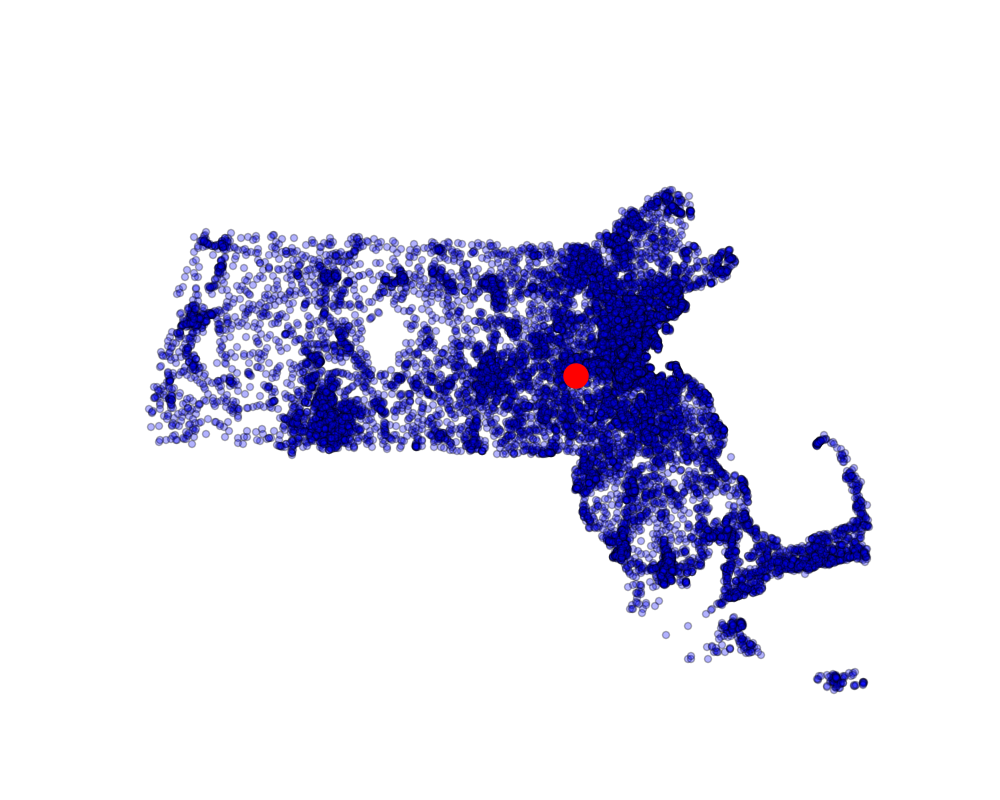
\includegraphics[width=5.5cm]{images/linweight.png} }}%
  \qquad
  \subfloat[$w(\xi)=\sqrt{\xi}$]{{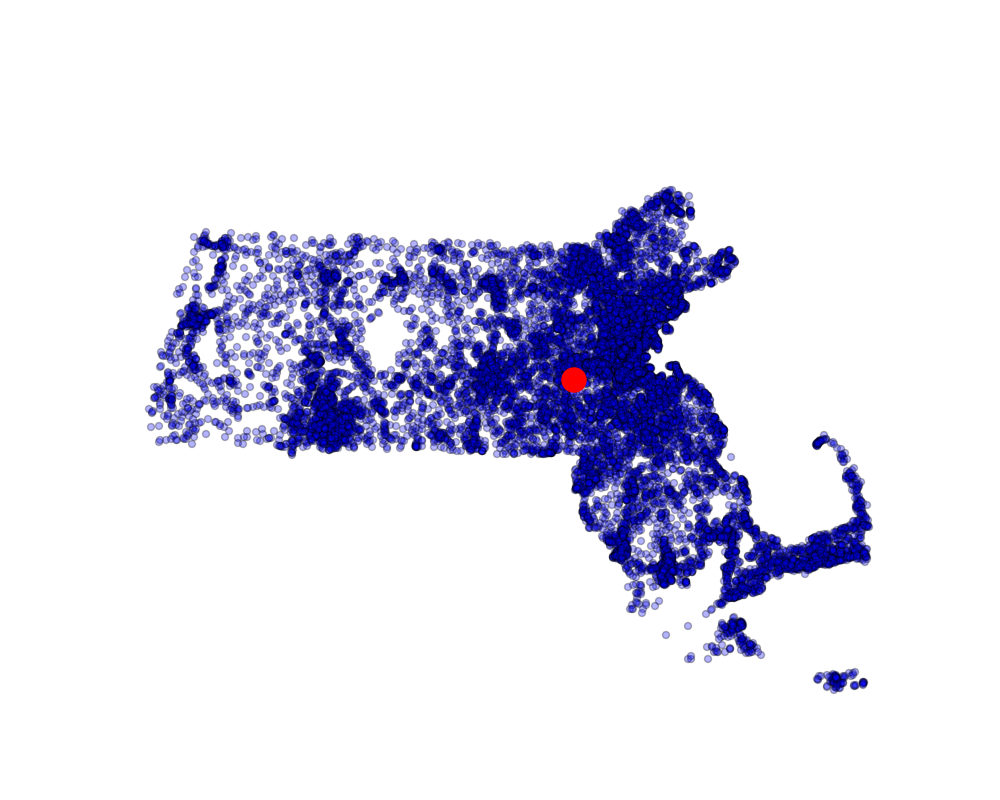
\includegraphics[width=5.5cm]{images/sqrtweight.png} }}%
  \qquad
  \subfloat[$w(\xi)=\xi^2$]{{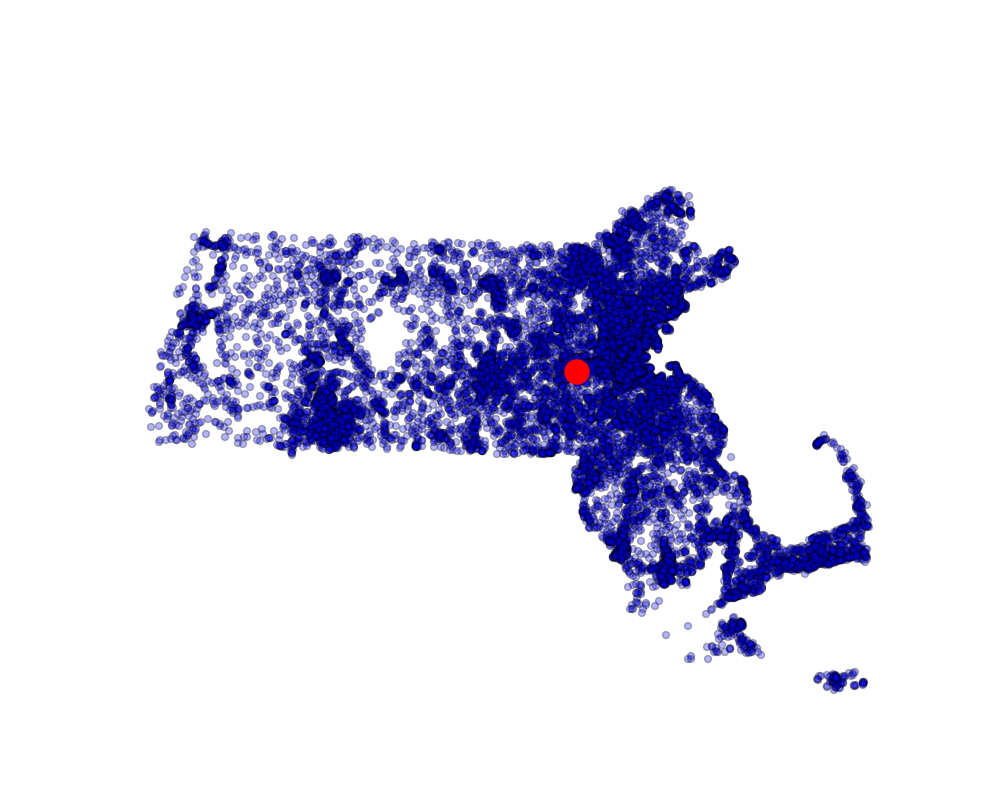
\includegraphics[width=5.5cm]{images/sqweight.png} }}%
  \qquad
  \subfloat[$w(\xi)=1$]{{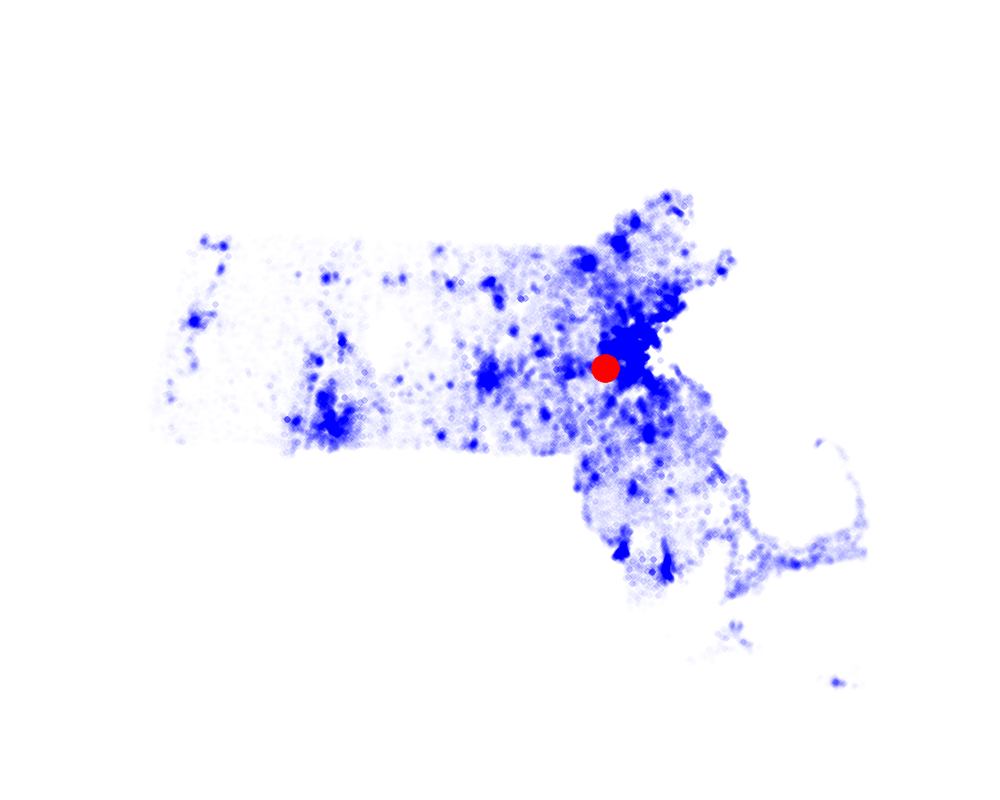
\includegraphics[width=5.5cm]{images/noweight.png} }}%
  \qquad
  \subfloat[][$w(\xi)=\begin{cases}\xi, & \xi > 1\\ 0, & \text{otherwise} \end{cases}$]{{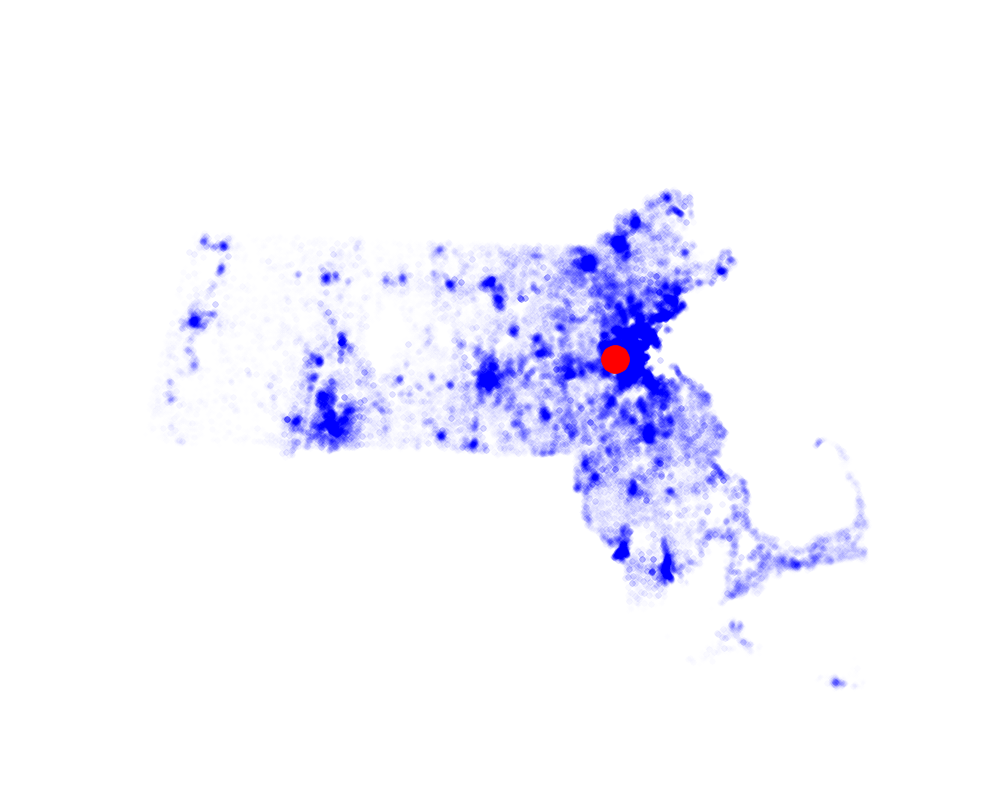
\includegraphics[width=5.5cm]{images/thresholdweight.png} }}
  \caption{Distribution center placement under various weighting \\ functions. The centers are shown in red.}
  \label{fig:popscale}
\end{figure}

When $k=1$, the weighted $k$-centers problem is easily solved via compass search. Compass search is a simple method of minimizing a function $f : \R^n \rightarrow \R$ that does not require computation of the gradient. The general structure of the algorithm is as follows: Starting from a starting location and with an initial step size and a set of directions that form a positive spanning set of $\R^n$, find a direction for which moving by the step size decreases the function and execute that step. If there is no such direction, decrease the step size and search anew for a direction that decreases the function. The algorithm terminates when the step size falls below a given tolerance. A more detailed description is given in Algorithm \ref{alg:compass} (see \cite{survey} for further details and proof of convergence). Compass search is susceptible to convergence within local extrema, which is usually avoided by running the search several times with randomly chosen starting points to more fully explore the space of possible solutions.

As above, we choose $f$ to be

$$\frac{\sum_i w(\xi_i) d(c, p_i)}{|\X|}.$$

Figure \ref{fig:popscale} shows distribution center placement for various $w$. As expected, the distribution center is consistently placed near Boston. Under $w(x) = \sqrt{x}$, the center moves farther away from Boston as the influence of high population to the objective function is decreased, and under $w(x) = x^2$, the center moves closer to the downtown neighborhoods of the city. However, the choice of weighting function appears to have little effect on placement of the center. Even when population is not taken into account, the center remains fairly close to Boston by virtue of the large number of census blocks located there.

This method works well for one distribution center, but the number of directions to search grows quickly with the number of centers.  Consider the case of $n$ clusters $c_1, ..., c_n \in \R^2$. Our function to minimize is now the full weighted mean distance function

$$\frac{\sum_i w(\xi_i) \min_{c \in \C} d(p_i, c)}{|\X|}$$

A positive spanning set for $\R^n$ must contain at least $n+1$ vectors \cite{charles}, so we must consider up to three possible directions at each step for each $p_i$. Determining the exact number of directions that must be searched for $n$ points in order to guarantee convergence to some maximum is beyond the scope of this report. Suffice it to say that better, more scaleable methods exist. One such algorithm is Lloyd's algorithm, a variant of which is described in the next section.

\begin{algorithm}
  \caption{Compass Sort}
  \label{alg:compass}
\begin{algorithmic}
  \STATE  Let $\lambda_1,...,\lambda_m$ be a positive spanning set of $\R^n$. Choose a starting guess $p_0$, a step size $s_0$, a scaling constant $\alpha<1$, and a tolerance $t$.
  \WHILE{$s_k > t$}
  \IF{$f(p_k + s_k\lambda_i) < f(p_k)$ for some $\lambda_i$}
  \STATE $p_{k+1} = p_k + s_k\lambda_i$
  \STATE $s_{k+1} = s_k$
  \ELSE
  \STATE $p_{k+1} = p_{k}$
  \STATE $s_{k+1} = \alpha s_k$
  \ENDIF
  \ENDWHILE
  \RETURN $p_{k+1}$
\end{algorithmic}
\end{algorithm}

\section{Multiple Distribution Centers} \label{multicenters}
Lloyd's algorithm provides a more scaleable solution for multiple distribution centers. This algorithm was originally applied to problems in information theory \cite{lloyd}, but has been adapted to other fields such as clustering. A detailed description is given in Algorithm \ref{alg:lloyd} (see \cite{kmeans} for further details).The general algorithm works as follows: first, assign, via some method, starting locations for the centers $c_i$. Then, assign each center $c_j$ a cluster $\Gamma$ of points that are closer to $c_j$ than to any other $c_k, \ \ j\neq k$. Next, adjust the location of the $c_i$ to the centers of their respective clusters. Repeat until the $c_i$ do not move between iterations.

In the unweighted problem, the centers of the clusters can be computed by taking the mean of each component of  the points in the cluster. In the weighted problem, this method does not work, since the center of the cluster has become a weighted mean of the points. Instead, in the center adjusting step, we find the new location for a center $c_j \in \Gamma$ by solving the optimization problem

$$\argmin_{c_j} \sum_{\{i: p_i \in \Gamma\}} w(\xi_i) d(p_i, c_j)$$

This is equivalent to finding a root of the gradient

$$\Bigg[ \sum_{\{i: p_i \in \Gamma\}} w(\xi_i) \Big(\frac{p_{i,x} - c_{j,x}}{d(p_i, c_j)}\Big), \sum_{\{i: p_i \in \Gamma\}} w(\xi_i) \Big(\frac{p_{i,y} - c_{j,y}}{d(p_i, c_j)}\Big) \Bigg]^T$$

We randomly assign starting centers, though other initialization methods may be used. This suffices to find a solution for an arbitrary number of distribution centers.

To find a solution such that the cost function is below a given threshold and the number of centers is minimized, run the algorithm for $1, 2, ..., k, ...$ centers until the cost function falls below the threshold. Lloyd's algorithm is not guaranteed to produce a global minimum, so to more fully explore the space, we run the algorithm several times, stochastically varying the initialization points, for each choice of $k$.

\begin{algorithm}
  \caption{Lloyd's Algorithm with Weighting}
  \label{alg:lloyd}
\begin{algorithmic}
  \STATE  Randomly choose $n$ initial centers $\{c_1^1, ..., c_n^1\}=\C$, and let $\{\gamma_1, ..., \gamma_n\}=\Gamma$ be their corresponding clusters. 
  \WHILE {$\exists c_i : c_i^k \neq c_i^{k-1}$}
  \FOR{$\gamma_i \in \Gamma$}
    \STATE $\gamma_i = \{x \in \X : d(x, c_i^k) < d(x, c_j^k) \ \forall j \neq i\}$
  \ENDFOR
  \FOR{$c_i \in \C$}
    \STATE $c_i^k = \argmin_{\chi} \sum_{\{i : p_i \in \gamma\}} w(\xi_i) d(p_i, \chi)$
  \ENDFOR
  \ENDWHILE
\end{algorithmic}
\end{algorithm}

\section{Experiments} \label{experiments}

As in the case of one distribution center, we test our algorithm on U.S. census data from Massachusetts. However, each time a clustering is finalized, there is no guarantee that the points in a single cluster will remain in that same cluster after the next iteration. This is particularly true when comparing the final product of two clusterings produced by different weighting functions, when the structure of the clustering and the centers themselves can differ widely. 

The primary motivation for experimentation with our augmentation of Lloyd's algorithm is two-fold. First, we are interested in reducing the validation error. Second, we are interested in characterizing the effect different weighting functions have on center placement. To investigate the reduction of validation error we examined the effect of adding more clusters to the data as well as the effect of filtering out smaller census blocks. The reasoning behind filtering the data by neglecting smaller population blocks is to speed up the adjustment of the centers as we fully bias the solution toward the higher population areas. 

We attempted to compare the results of different clusterings (beyond the rescaling of the $w(\xi_i)$, as done for Section \ref{rescale}) produced by each weighting function by comparing each clustering against an independent subset of the data held out from the points the clusters optimized over. This led to a partition of our dataset into a randomly distributed test and validation set, with an 85/15 splitting. The reason for having a dedicated validation set is that the clusters will have been defined and optimized based on the test set, altering the cost function over the surface of population points from cluster to cluster. The validation set is then used to serve as a means to check whether our newly determined clustering also minimizes the distance between this independent set of points. This also allows us to examine the robustness of our algorithm to the vagaries of real data. Our goal is to produce a choice of center placement that could be used in real-world applications, and testing it on an independent set acknowledges the fact that there would be differences in collected data and actual data due to movement of populations, data collection errors, etc.

We encountered significant difficulties when attempting to compare the different weight functions. In order to compare results with the same tolerance and different $w$, we develop a simple rescaling such that under each function $w$, all calculated weights satisfy $\{w(\xi_i) \in [0,1] \ \big| \ \sum_i w(\xi_i) = 1\}$. The calculated costs  scale with the order of the function, providing widely varying measures of performance for similar solutions with the same number of clusters. As discussed above as well as in Section \ref{rescale}, we scaled all $w$ to the same order of magnitude which provides a closer measure of the cost a certain clustering provides, thus facilitating general comparisons. Unfortunately, the magnitude of the cost function under the various weightings differs sufficiently to complicate comparisons between the cost of two clusterings.

\begin{figure}[!ht]%
  \centering
  \subfloat[$k=1$]{{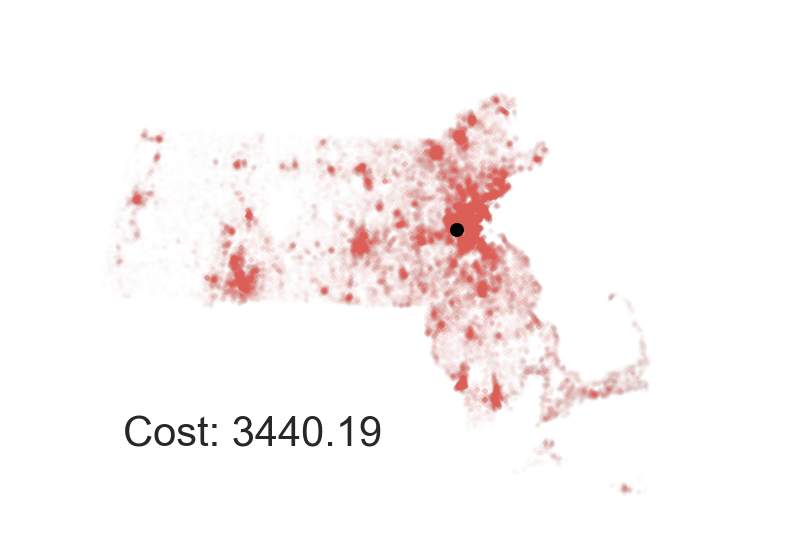
\includegraphics[width=5.5cm]{images/linwt_comparison1.png} }}%
  \qquad
  \subfloat[$k=2$]{{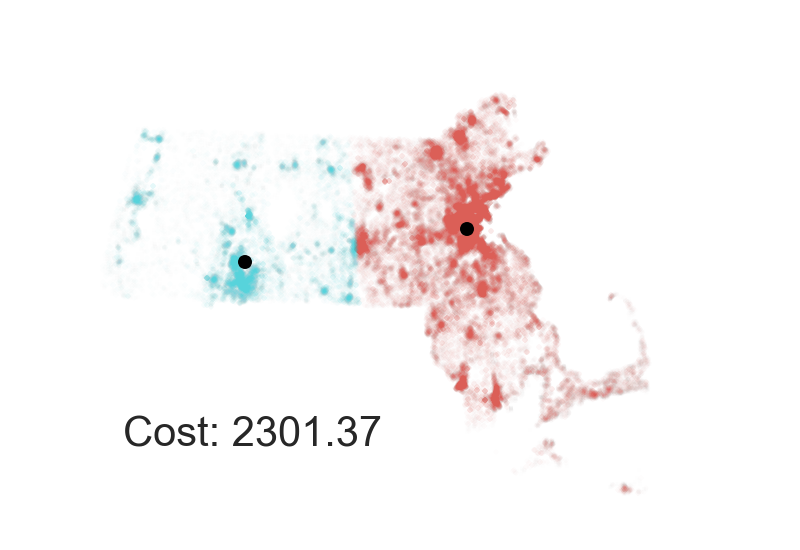
\includegraphics[width=5.5cm]{images/linwt_comparison2.png} }}%
  \qquad
  \subfloat[$k=3$]{{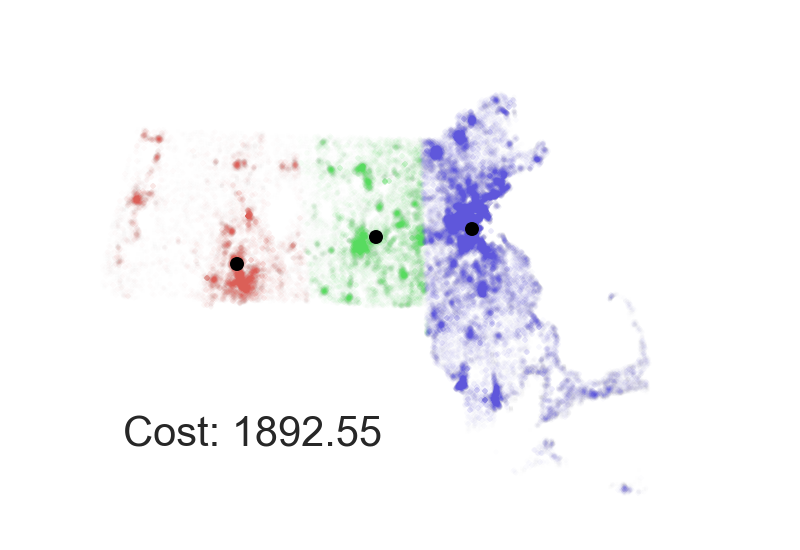
\includegraphics[width=5.5cm]{images/linwt_comparison3.png} }}%
  \qquad
  \subfloat[$k=4$]{{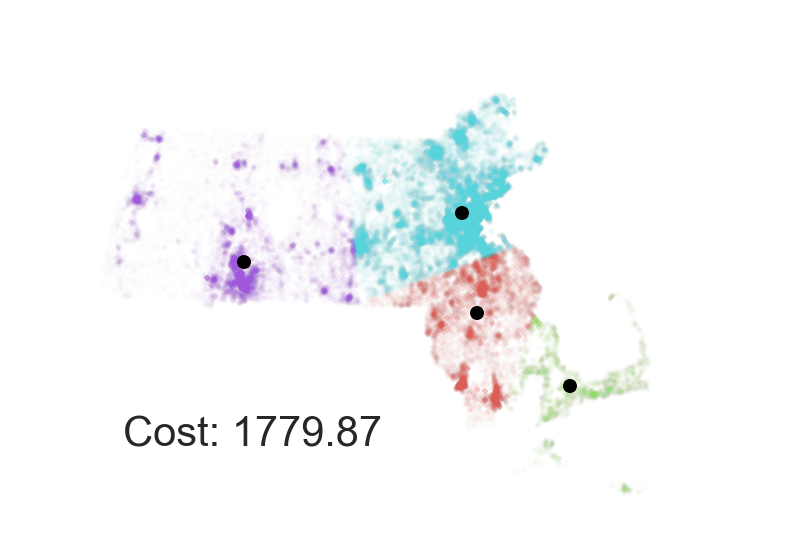
\includegraphics[width=5.5cm]{images/linwt_comparison4.png} }}%
  \qquad
  \subfloat[$k=5$]{{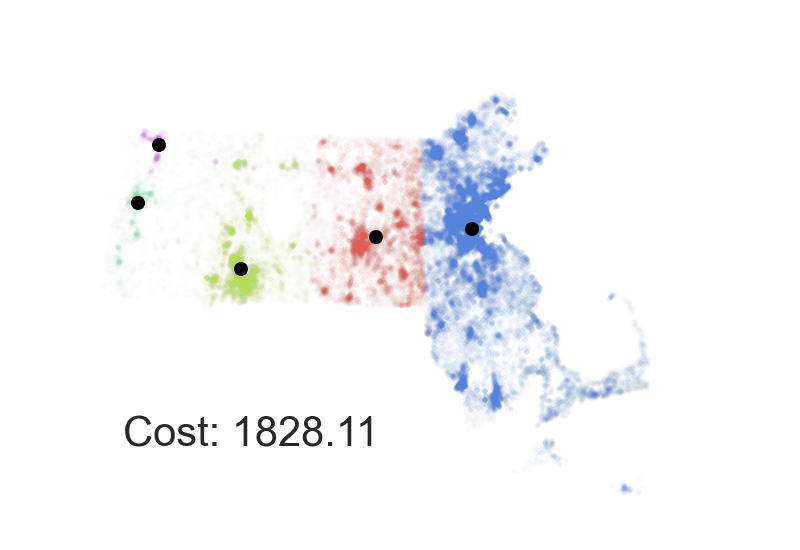
\includegraphics[width=5.5cm]{images/linwt_comparison5.png} }}%
  \caption{Distribution center placement and validation cost under linear weighting for $k=1,...,5$. The cost function is shown, and centers are in black.}
  \label{fig:10centers}
\end{figure}

 \subsection{Effect of Number of Centers on Cost}
Figure \ref{fig:10centers} shows the cluster arrangements for unscaled linear weighting for $k=1,...,10$ clusters. Also shown in figure \ref{fig:centersvscost} is the validation cost as a function of number of clusters.


\begin{figure}[!ht]%
  \ContinuedFloat
  \centering
  \subfloat[$k=6$]{{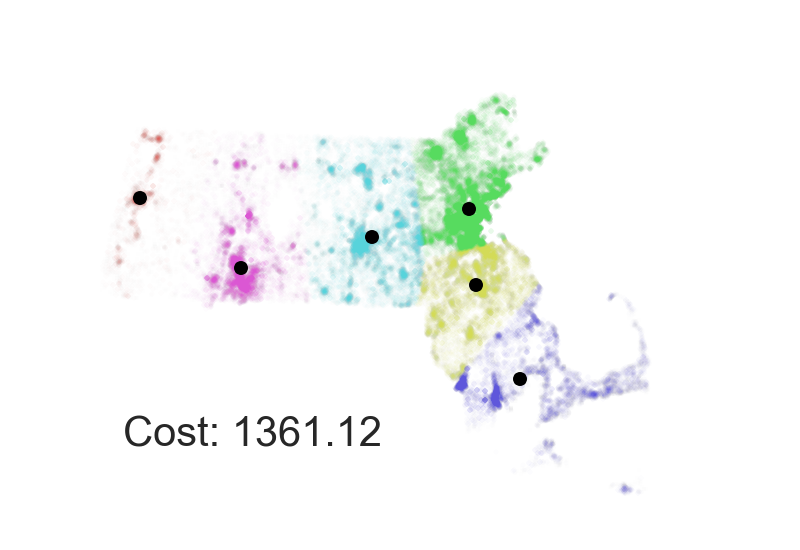
\includegraphics[width=5.5cm]{images/linwt_comparison6.png} }}%
  \qquad
  \subfloat[$k=7$]{{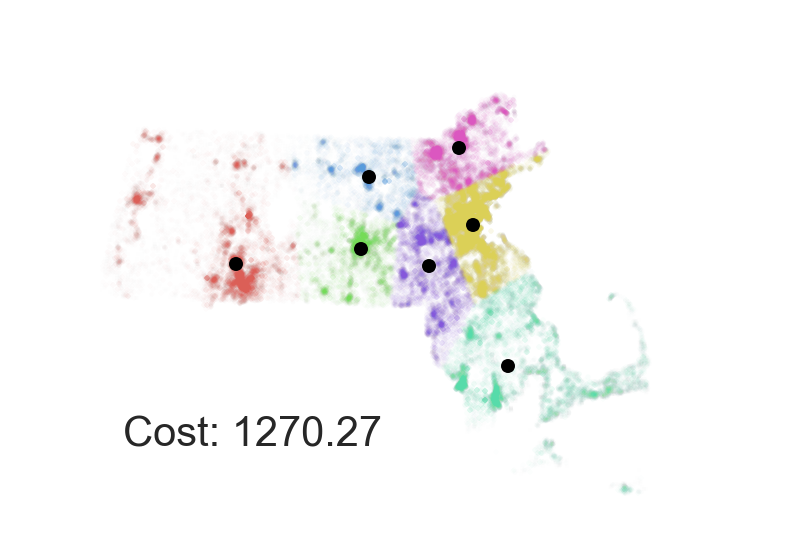
\includegraphics[width=5.5cm]{images/linwt_comparison7.png} }}%
  \qquad
  \subfloat[$k=8$]{{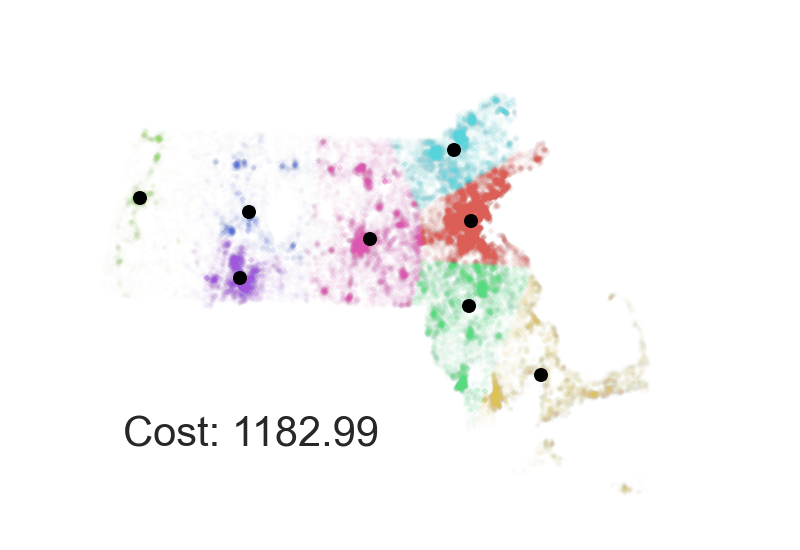
\includegraphics[width=5.5cm]{images/linwt_comparison8.png} }}%
  \qquad
  \subfloat[$k=9$]{{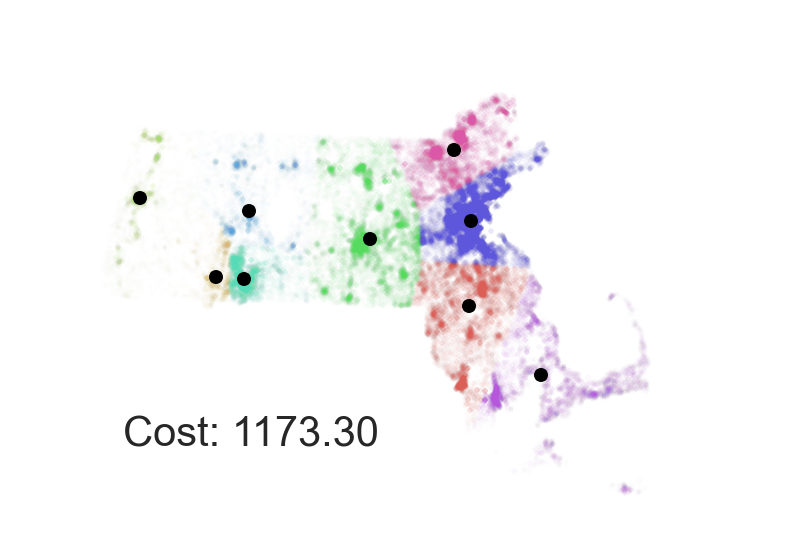
\includegraphics[width=5.5cm]{images/linwt_comparison9.png} }}%
  \qquad
  \subfloat[$k=10$]{{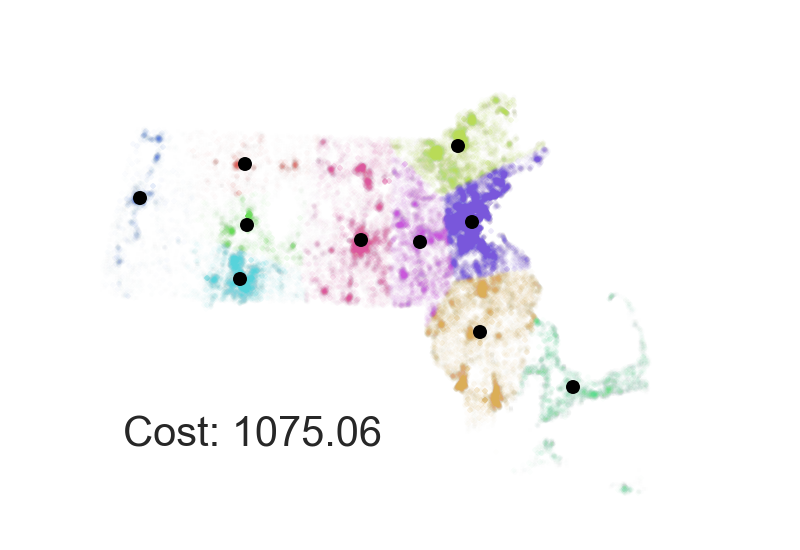
\includegraphics[width=5.5cm]{images/linwt_comparison10.png} }}%
  \caption{Distribution center placement and validation cost under linear weighting for $k=6,...,10$. The cost function is shown, and centers are in black.}
  \label{fig:10centers}
\end{figure}

 
As expected, centers are consistently located near urban areas. Also as expected, cost decreases, albeit erratically, with the number of centers. The five center arrangement, for example, results in higher cost than the four center arrangement, this is likely due to the random initialization of the centers. Had time permitted, performing multiple runs and then averaging their results would have produced a smoother curve with fewer unexpected results. Nonetheless, the results are consistent with expectations.

\subsection{Effect of Population Filtering on Cost}
Figure \ref{fig:threshold} shows the effects of population filtering on center placement for selected population thresholds. Recall that a population filter of $n$ means that points, and corresponding weights, with population less than $n$ are neglected when adjusting the cluster centers $c_i$. All thresholds were tested with five clusters.

The results are not surprising. Increasing the threshold does not have a significant effect on placement of centers on a micro level. For instance, the clusters containing Boston and Springfield, respectively, are always in roughly the same places. A sufficiently high threshold does serve to all but ignore less populated areas. When using a population filter of 100, the Boston cluster contains the entirety of southeastern Massachusetts and the cape, moving those cluster centers to the northeast and western regions of Massachusetts. At lower filter levels, the clustering is not greatly affected outside of slight variations of the centers around the major population regions while computation time of the full solution decreases. There appears to be an optimal filtering threshold in the interval [30, 50] below which center placement and cost are not greatly affected. A filter greater than 100 certainly biases the solution sufficiently to raise concerns about the applicability of the proposed clusterings to the unfiltered data, with approximately $50\%$ of the census data points neglected by such a filter.

\begin{figure}[!ht]%
  \centering
   \subfloat{{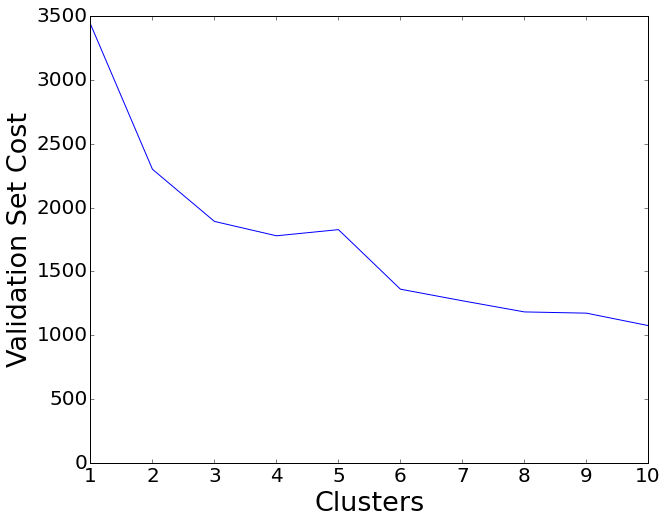
\includegraphics[width=5.5cm]{images/validationcost.png} }}%
   \caption{Validation cost vs. number of clusters}
   \label{fig:centersvscost}
 \end{figure}
 
\begin{figure}[!ht]%
  \centering
  \subfloat[Filter of 10]{{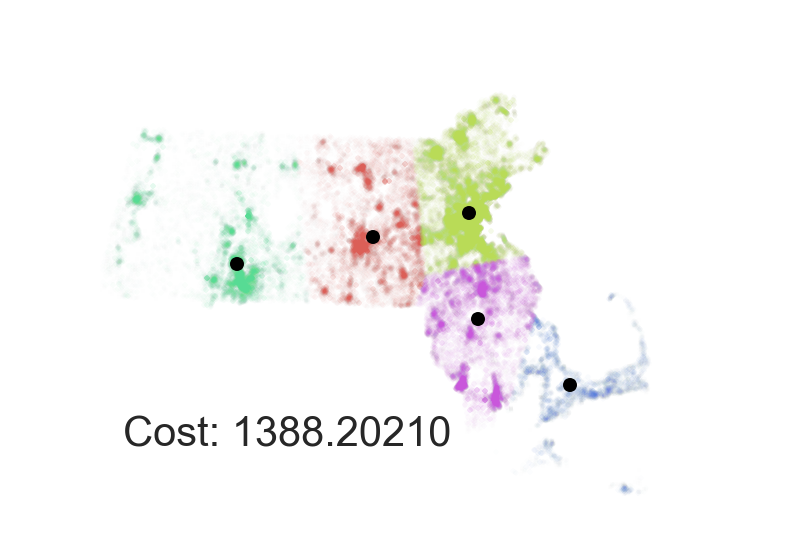
\includegraphics[width=5.5cm]{images/solution_linwt_clusters5_minpop10.png} }}%
  \qquad
  \subfloat[Filter of 25]{{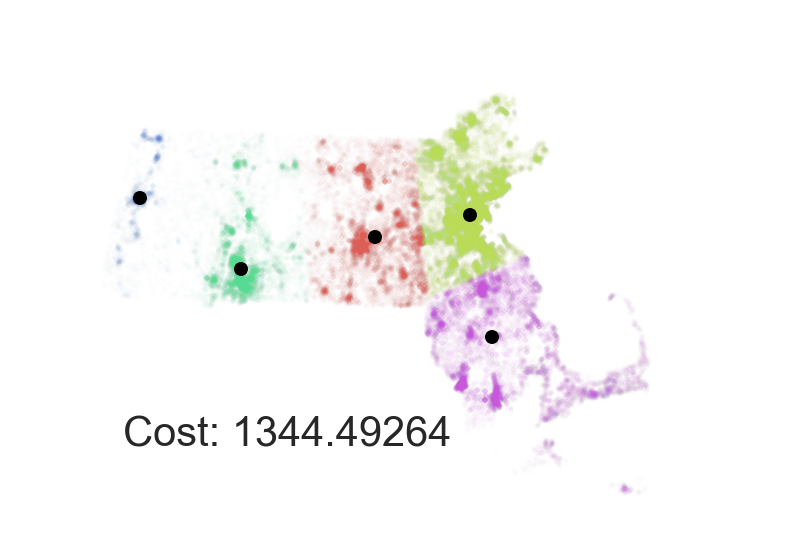
\includegraphics[width=5.5cm]{images/solution_linwt_clusters5_minpop25.png} }}%
  \qquad
  \subfloat[Filter of 50]{{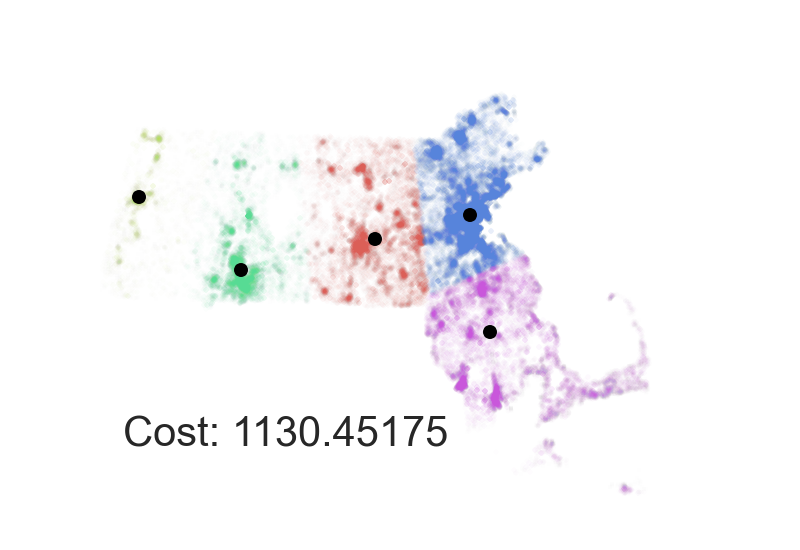
\includegraphics[width=5.5cm]{images/solution_linwt_clusters5_minpop50.png} }}%
  \qquad
  \subfloat[Filter of 75]{{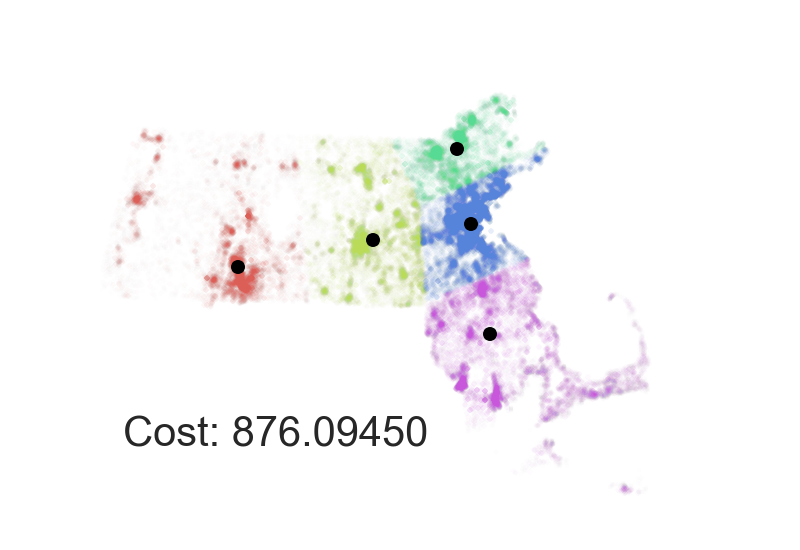
\includegraphics[width=5.5cm]{images/solution_linwt_clusters5_minpop75.png} }}%
  \qquad
  \subfloat[Filter of 100]{{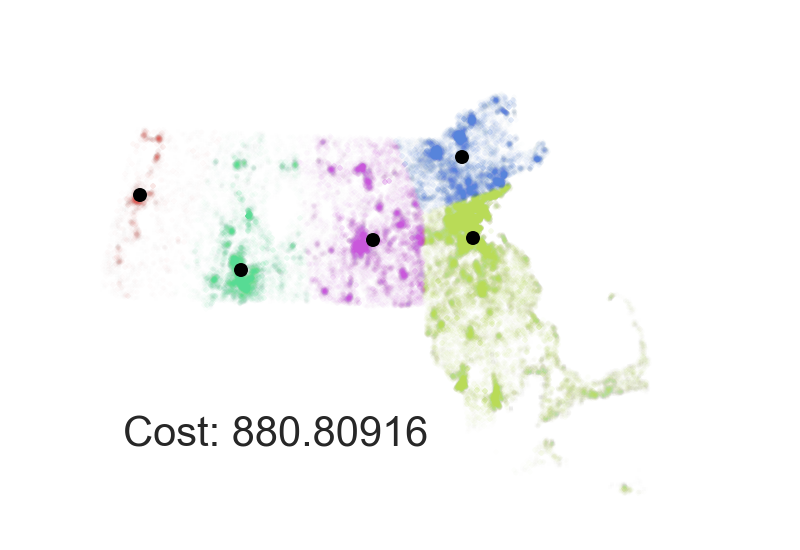
\includegraphics[width=5.5cm]{images/solution_linwt_clusters5_minpop100.png} }}%
  \caption{Distribution center placement under linear weighting for various population filters. The cost function is displayed, and centers are in black.}
  \label{fig:threshold}
\end{figure}

\subsection{Comparison of Weighting Functions}
\begin{figure}[!ht]%
  \centering
  \subfloat[$w(\xi)=\xi$]{{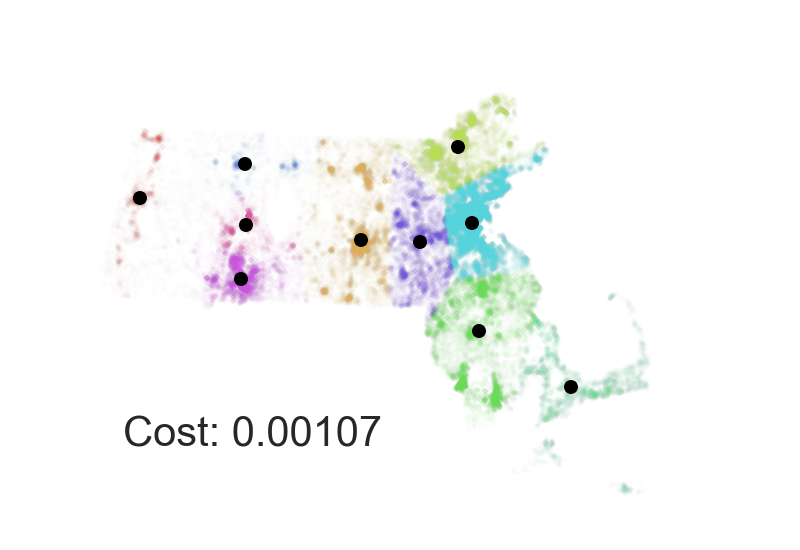
\includegraphics[width=5.5cm]{images/solution_linwt_clusters10_minpop1.png} }}%
  \qquad
  \subfloat[$w(\xi)=\sqrt{\xi}$]{{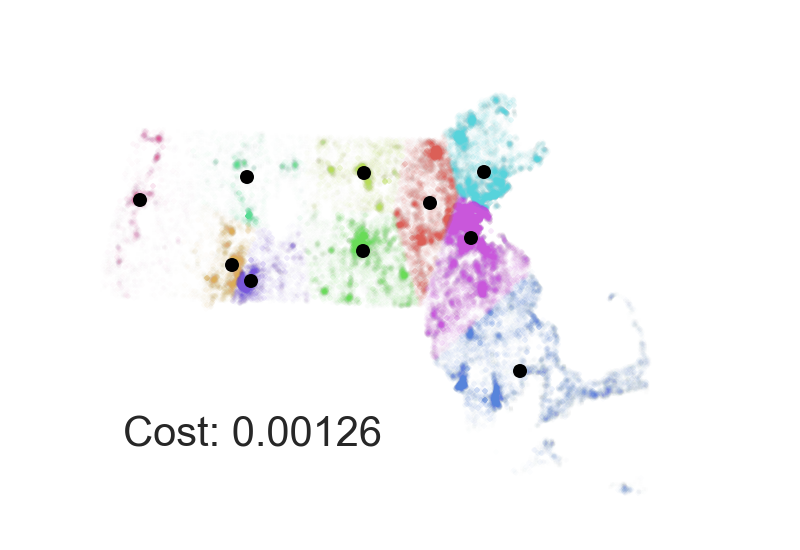
\includegraphics[width=5.5cm]{images/solution_sqrtwt_clusters10_minpop1.png} }}%
  \qquad
  \subfloat[$w(\xi)=\xi^2$]{{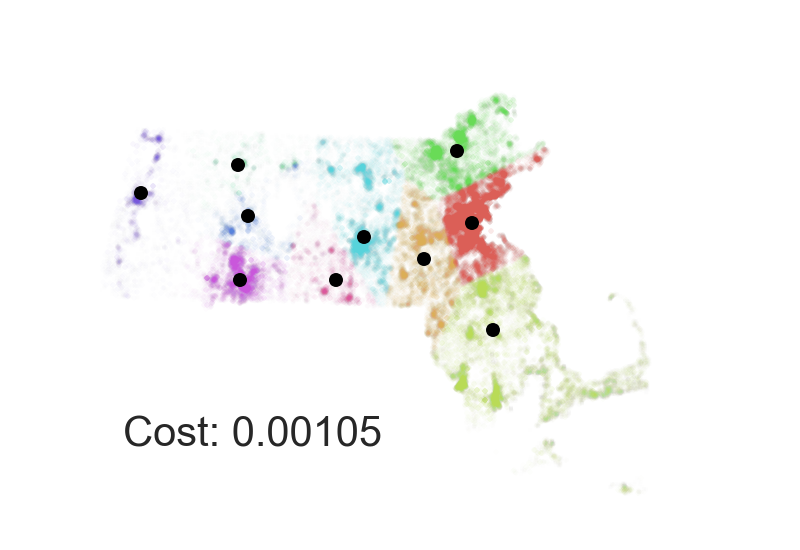
\includegraphics[width=5.5cm]{images/solution_sqwt_clusters10_minpop1.png} }}%
  \qquad
  \subfloat[$w(\xi)=\log(\xi)$]{{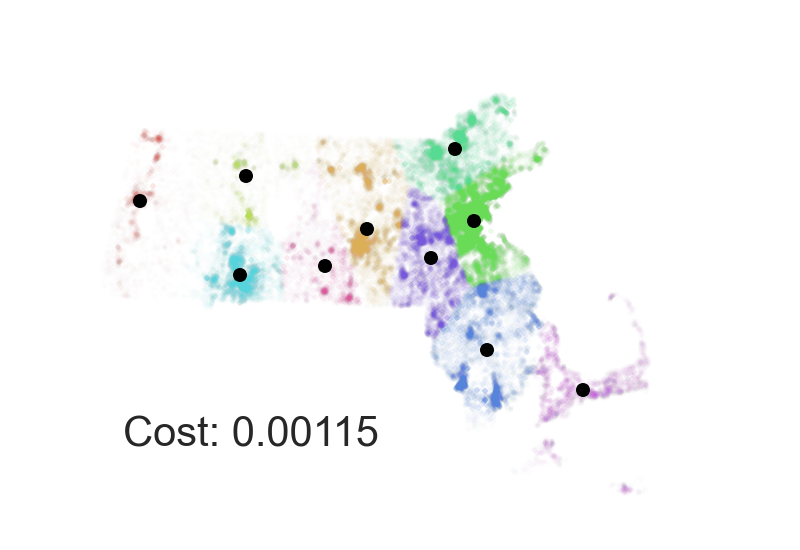
\includegraphics[width=5.5cm]{images/solution_logwt_clusters10_minpop1.png} }}%
  \qquad
  \subfloat[$w(\xi)=\frac{\xi}{max_j \xi}$]{{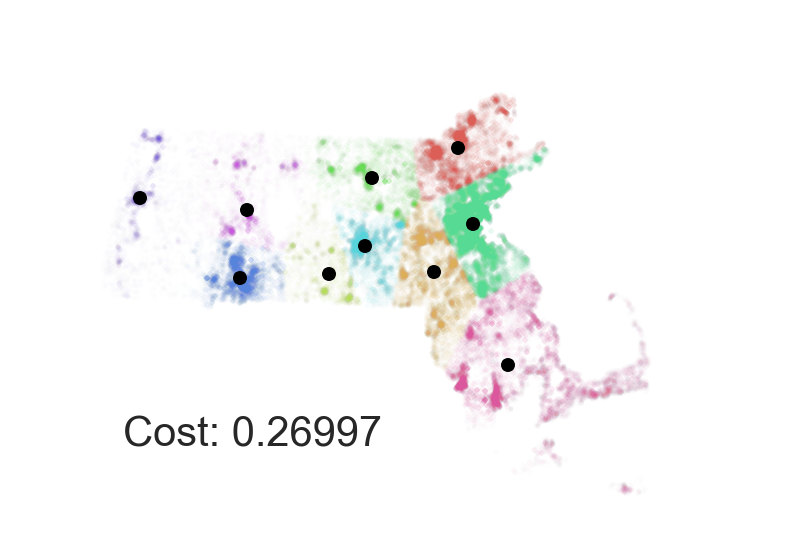
\includegraphics[width=5.5cm]{images/solution_maxwt_clusters10_minpop1.png}}}%
  \caption{Distribution center placement under various weighting functions. The value of the cost function is displayed, and centers are shown in black.}
  \label{fig:weightcomp}
\end{figure}

\subsubsection{Rescaling}\label{rescale}
Without rescaling, it is difficult to compare results with different choices of $w$. For example, the weighted mean distance with $w(\xi) = \xi^2$ will necessarily be much greater than the weighted mean distance with $w(\xi) = \sqrt{\xi}$. Therefore, we divide both the tolerance and the cost function by

$$\sum_i w(\xi_i)$$

This roughly corresponds to a rescaling to the same scale of the case when $w(\xi) = \xi$. Effectively, all weights satisfy $\{w(\xi_i) \in [0,1] \ \big| \ \sum_i w(\xi_i) = 1\}$ after rescaling. Rescaling the tolerance is equivalent to choosing a smaller tolerance to start with. However, rescaling is a systematic way of converting a tolerance with a physical interpretation to one suited to the problem. 

\subsubsection{Results} \label{results}
Figure \ref{fig:weightcomp} shows the results of generating 10 clusters under four different weighting functions other than the default linear function that was demonstrated above. As in the case of one distribution center, choice of weighting function has little effect on center location. Log weighting, which curbs the influence of points with high population, does not show substantially different center placement from square weighting, which increases the influence of high population. It is possible that this behavior is a result of some non-general aspect of our problem, such as the population distribution and density of Massachusetts, or the discrete and often highly spread out distribution of points, but in our case, the weighting function has little effect on center placement.

The results of clustering under the influence of different weight functions suggest intuition behind the cases in which one choice of $w$ could be more advantageous than another. A superlinear $w$ could be used in a situation in which it is not as useful to place distribution centers near areas of low population density; for example, an expensive specialty store might place great importance on serving urban areas. A sublinear $w$ could be used in a situation in which optimally serving areas of high population density is not important, as in the case of a big-box retailer that customers visit infrequently. Such comparisons could be useful when considering the expense of procuring land in relation to the geographic distribution of the demographic that you hope to serve with your distribution center.

\section{Conclusions \& Future Work}
\subsection{Conclusions}
As expected, placing distribution centers near areas with high population density is optimal. This is hardly surprising, though it serves as a good sanity check for our algorithm. More centers leads to a lower cost function, though the decrease slows as the number of centers increases. The marginal utility of adding extra centers decreases rapidly, as is readily apparent with as few as 10 centers.

The choice of weight function, out of the ones we tested, appears to have little impact on center placement. More extreme choices, such as $w(\xi)=2^{\xi}$, could drastically alter center placement, and weight functions that \textit{penalize} large populations, such as $w(\xi)=\frac{1}{\xi}$, could result in centers placed as far from cities as possible, though examining their effects is not the focus of this paper.

Population filters below a certain threshold also had little effect on center placement, though more extreme filters moved centers even closer to major cities. This is promising, since as mentioned above, as many as 30\% of points could be removed with little effect on the results, but a significant improvement in speed. Since we have observed our weighted Lloyd's algorithm to be rather slow, this could be a useful tactic when analyzing large datasets.
 
\subsection{Future Work}
The choice of weighting function is a potential area of further study. Though the choice of weighting function did not significantly impact our results, it could have a greater influence in other situations. We assume that the weighting function is chosen based on \textit{a priori} domain knowledge, which suggests an investigation into data-driven choices of weighting functions for known business problems. Also of interest are exotic functions that transform population counts in extreme or unusual ways such as those mentioned above.

Another interesting future variation that lends itself to study is how the clustering changes with the granularity of the population data. We utilized US Census\cite{census} block data that, while sufficiently detailed for a macro analysis of Massachusetts, is not detailed enough to provide adequate insight for the optimal location of distribution and/or retail centers within a densely populated city. If we had access to parcel data (storefronts and other properties at the street level) it is likely that our clustering solution would be fundamentally different from those presented in this paper.

A better rescaling function would allow more direct comparison between weighting methods. With our na\"ively chosen rescaling, the cost function is still much lower for sublinear $w$ than for linear or superlinear $w$, which complicates performance comparisons, since it is not obvious how to compare an inherently lower cost function to an inherently higher one. With a better rescaling process, it might be possible to numerically compare the performance of the various weighting functions in figure \ref{fig:weightcomp} against each other, rather than simply looking at how the centers change.

Balancing the cost of placing a distribution center with the cost of serving customers poorly is an interesting variant of the problem we consider. Given a center placement method, such as the one we developed, one could find $\C$ to minimize 
$$\frac{\sum_i w(\xi_i) \min_{c \in \C} d(p_i, c)}{|\X|} + f(|\C|)$$
where $f$ is a function that represents the cost of building and maintaining more distribution centers. 

Perhaps the most important future work is in empirically examining and categorizing performance, speed, and convergence of Lloyd's algorithm when applied to weighted problems like weighted $k$-centers. We made many unsupported assumptions in our work, such as the assumption that randomly choosing starting points is a good strategy, and a more thorough investigation could examine, among other things, which assumptions are valid and which should be replaced.

\begin{thebibliography}{99}
  \bibitem{kmeans}
  Kanungo, T., Mount, D. M., Netanyahu, N. S., Piatko, C., Silverman, R., and Wu, A. Y (2002). An Efficient $k$-Means Clustering Algorithm: Analysis and Implementation. \textit{IEEE Transactions on Pattern Analysis and Machine Intelligence 24}(7), pp. 881-892.
  \bibitem{lloyd}
  Lloyd, S. P (1982). Least Squares Quantization in PCM. \textit{IEEE Transactions on Information Theory 28}(2), pp. 129-137.
  \bibitem{census}
  U.S. Census Bureau. \textit{TIGER/Line� with Selected Demographic and Economic Data: Population \& Housing Unit Counts}. Retrieved from https://www.census.gov/geo/maps-data/data/tiger-data.html
  \bibitem{survey}
  Kolda, T. G., Lewis, R. M., and Torczon, V (2003). Optimization by Direct Search: New Perspectives on Some Classical and Modern Methods. \textit{SIAM Review, 45}(3), pp. 385-482.
  \bibitem{charles}
  Davis, C. (1954). Theory of Positive Linear Dependence. \textit{Journal of American Mathematics, 76}(4), pp. 733-746.
  \bibitem{pyshp}
  \textit{Python Shapefile Library}. Github repository. Retrieved from https://github.com/GeospatialPython/pyshp
  \bibitem{1D}
  Chen, D. Z., Li, J., and Wang, H. Efficient Algorithms for the One-Dimensional $k$-Center Problem (2015). \textit{Theoretical Computer Science 592}, pp. 135-142.
  \bibitem{blocks}
  Rossiter, K. (2011, July 20). What are census blocks? [Web log post]. Retrieved from http://blogs.census.gov/2011/07/20/what-are-census-blocks/
  \bibitem{weightedclustering}
  Ackerman, M., Ben-David, S., Br\^anzei, S., and Loker, D (2012). Weighted Clustering. \textit{Proceedings of the Twenty-Sixth AAAI Conference on Artificial Intelligence}.
  \bibitem{crystal}
  Bourne, D., and Roper, S (2014). Centroidal Power Diagrams, Lloyd's Algorithm, and Applications to Optimal Location Problems. \textit{SIAM Journal on Numerical Analysis, 53}(6).
\end{thebibliography}
\end{document}